\section{Theorie}

Damit das System auch in bereits bestehenden Solaranlagen eingebaut werden kann um fehlerhafte Solarpanel zu detektieren, muss die Datenübertragung ohne weitere Verkabelung möglich sein. Die einfachste Art dies ohne grossen Energieaufwand zu bewerkstelligen ist durch eine direkte Übertragung via Kabel. Die Powerline-Kommuni"-kation bildet somit die wichtigste Grundlage für das Projekt, weshalb sie in diesem Kapitel ausführlich erklärt wird. 


Ohne zusätzliche Kabel soll das Signal über die Powerline übertragen werden. Dafür wird das Signal moduliert und induktiv auf die Powerline eingekoppelt. Das zentrale Baustück dafür ist der ST7540, ein Powerline Transceiver der Signale auf die Powerline senden kann sowie auch imstande ist Signale zu empfangen. Die verwendete Modulationsart ist FSK (Frequency-Shift-Keying) die das zu übertragende Signal auf ein Trägersignal moduliert, in dem es die Frequenz des Trägersignals verändert. Dieses Prinzip ist in der Abbildung \ref{fig::fskDemo} ersichtlich.


\begin{wrapfigure}{l}{0.5\textwidth}
\centering
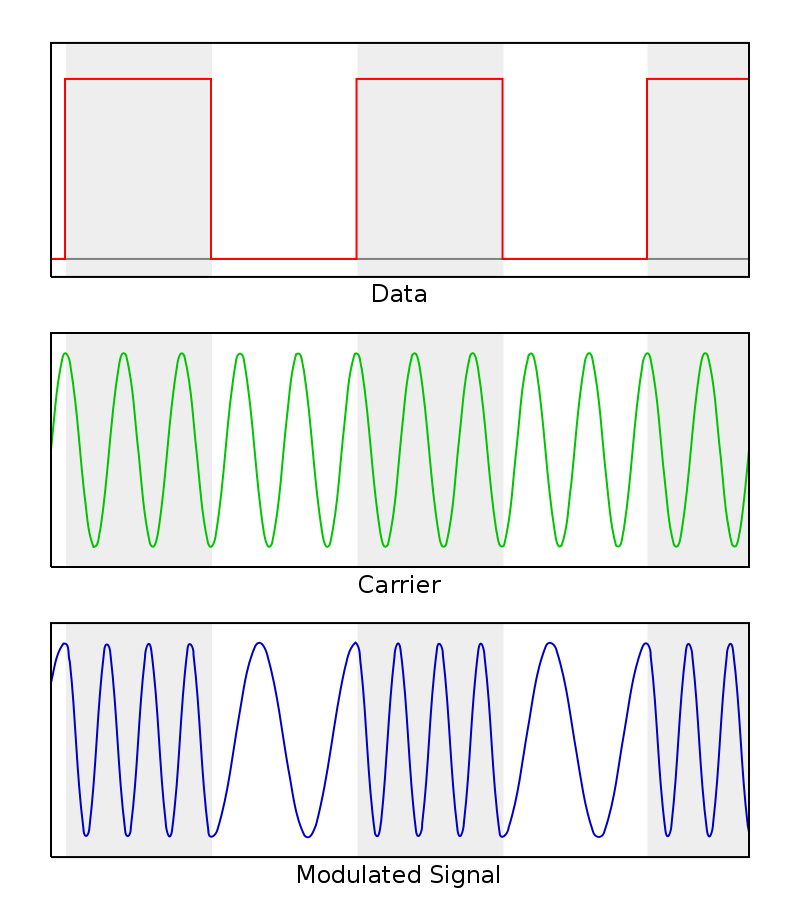
\includegraphics[width=0.5\textwidth]{FSK_demo.png}%
\caption{Prinzip der FSK Modulation \cite{fskDemo_wiki} }
\label{fig::fskDemo}
\end{wrapfigure}

%Die Beschaltung des Transceivers besteht aus drei Filtern, welche an die Übertragungsfrequenz angepasst werden müssen: Tx Aktiv Filter, Tx und Rx Passiv Filter. Zur Dimensionierung dieser wurde der Application Guide \cite{Applic_Guide_ST7540} sowie das Datenblatt \cite{Datasheet_ST7540}. Es sind indgesamt 8 Übertragungsfrequenzen im Bereich von 60-132.5kHz vorprogrammiert. Der ST7540 kann über SPI oder UART angesteuert werden (UART/SPI Pin), der Clock wird mit einem Quartz generiert (16MHz). Der Transceiver kann zwischen ``sending'' oder ``receiving'' umschalten:
Die Beschaltung des Transceivers besteht aus drei Filtern, die an die Übertragungsfrequenz angepasst werden müssen: Tx Aktiv Filter, Tx und Rx Passiv Filter. Zur Dimensionierung dieser wurde der Application Guide \cite{Applic_Guide_ST7540} sowie das Datenblatt \cite{Datasheet_ST7540} als Referenz genommen. Es sind indgesamt 8 Übertragungsfrequenzen im Bereich von 60-132.5kHz vorprogrammiert sowie 4 Baudraten: 600, 1200, 2400, 4800. Der ST7540 kann über SPI oder UART angesteuert werden (UART/SPI Pin), der Clock wird mit einem Quartz generiert (16MHz). Der Transceiver kann zwischen ``sending'' oder ``receiving'' umschalten:

\subsection{Receiving mode}
Der ``receive'' Modus ist aktiv wenn RxTx = 1 und REG\_DATA = 0. In diesem Modus liest der Powerline Transceiver die Informationen von der Powerline und überträgt diese an den Microkontroller. Der Powerline Transceiver verbraucht in diesem Modus einen sehr geringen Strom (ca.5mA).

Da die Kommunikation zwischen Sensorprint und Meldeprint unidirektional ist, wird dieser Modus nur beim Meldegerät gebraucht.

\subsection{Sending mode}
Der ``sending'' Modus ist aktiv wenn RxTx = 1 und REG\_DATA = 0. Die Daten werden entweder vom Control Register (SPI) oder direkt vom Tx Pin (UART) eingelesen. Die Daten werden dann moduliert und auf die Powerline gesendet. In diesem Modus hat der Powerline Transceiver einen hohen Leistungkonsum.

Dieser Modus wird nur auf den Sendeprints benutzt und werden mit UART angesteuert, weshalb auf das Control Register nicht zugegriffen wird. Das senden soll auch auf einem Minimum bleiben, da ein dauerhaftes Senden die Vorgabe von den durchschnittlichen 100mW nicht einhalten würde.



